\Chapter{REVUE DE LITTÉRATURE}\label{sec:RevLitt}

\section{Le disque d'Euler}
\subsection{Définition générale et lien avec la roue Cyr}
Le disque d'Euler est un disque plein semblable à une grosse pièce de monnaie. Son mouvement peut être découpé en deux phases:
\begin{itemize}
\item Phase 1, ou phase initiale: Le disque, incliné, roule sur sa tranche en suivant une trajectoire circulaire.
\item Phase 2, ou phase terminale: le disque se met à tourner de telle manière que le point de contact avec le sol se déplace de plus en plus lentement le long de son contour, un mouvement d'oscillation apparaît, accompagné d'un son vibratoire \cite{ringing}, et atteint sa fréquence maximale avant que le disque tombe à plat sur le sol.
\end{itemize}

C'est de la phase terminale, que le disque d'Euler tient sa popularité. Son côté spectaculaire en a fait un jouet éducatif, tandis que son comportement chaotique attise les curiosités scientifiques. Il a été déterminé que le comportement du disque au terme de cette phase était du à la viscosité de l'air.\\

\begin{figure}[h]
\centering
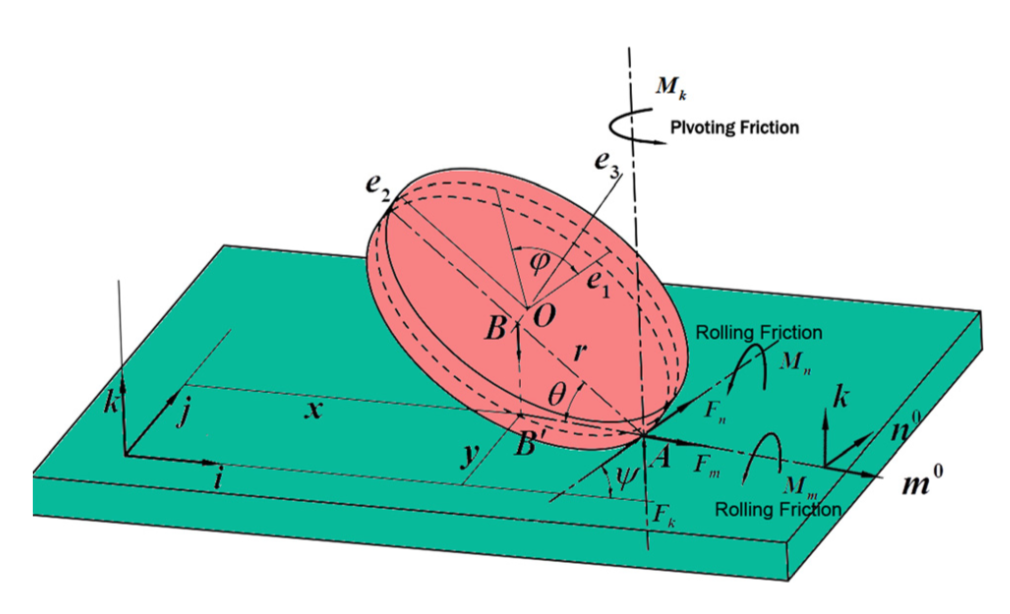
\includegraphics[width=200]{images_autres/diskma.png}
\caption{Modélisation du disque d'Euler en mouvement \cite{ma_dynamics_2016}.}
\label{fig:figures}
\end{figure}

La roue roule sur sa tranche en décrivant des cercles de plus en plus petits, avant d'entrer en phase terminale. Ces deux phases correspondent respectivement aux deux figures fondamentales de roue Cyr que sont la roue et la pièce, présentées à l'introduction. Il s'agit également de l'un des mouvements qu'on souhaite modéliser afin d'identifier les paramètres mécaniques et géométriques déterminants pour la stabilité dynamique et de caractériser leur influence. 

\subsection{Modèle mathématique et intégration numérique}
Campos et al \cite{campos} et Kessler et O'Reily \cite{ringing} développent des modèles mathématiques du disque d'Euler en vue d'une intégration numérique. Il caractérisent son comportement en termes de trajectoire du point de contact avec le sol, de variation d'énergie et de fréquence. 

\subsection{Étude de la stabilité en régime permanent}
Batista \cite{Batista} étudie la stabilité en régime permanent du mouvement du disque d'Euler correspondant à la phase 1. Il développe un modèle cinématique du disque et définit les conditions d'existence d'une position d'équilibre dynamique en fonction du signe de $\Omega_0^2$, la vitesse à laquelle le disque décrit des cercles en roulant. Ce signe dépend de l'angle d'inclinaison du disque, $\theta_0$ et du rayon des cercles décrits, $r$. Chaque couple $(\theta_0,r)$ permet de déterminer si l'équilibre dynamique est possible ou non. Avec un raisonnement similaire, Batista détermine si, en cas de stabilité, le système reste stable ou non lorsqu'on ajoute une petite perturbation. Le résultat final est une carte de stabilité d'abscisse $\theta_0$ et d'ordonnée $r_c$, où la couleur de chaque point correspond à un des trois cas: stable, indéfini (l'équilibre dynamique ne peut pas exister), ou instable en cas de perturbation.

\begin{figure}[h]
\centering
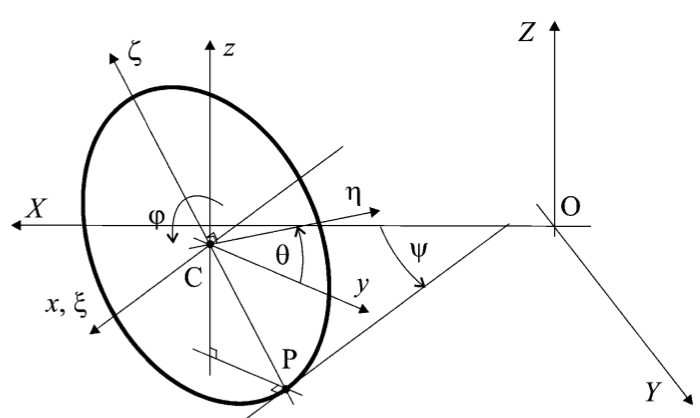
\includegraphics[width=200]{batista/ref1.png}
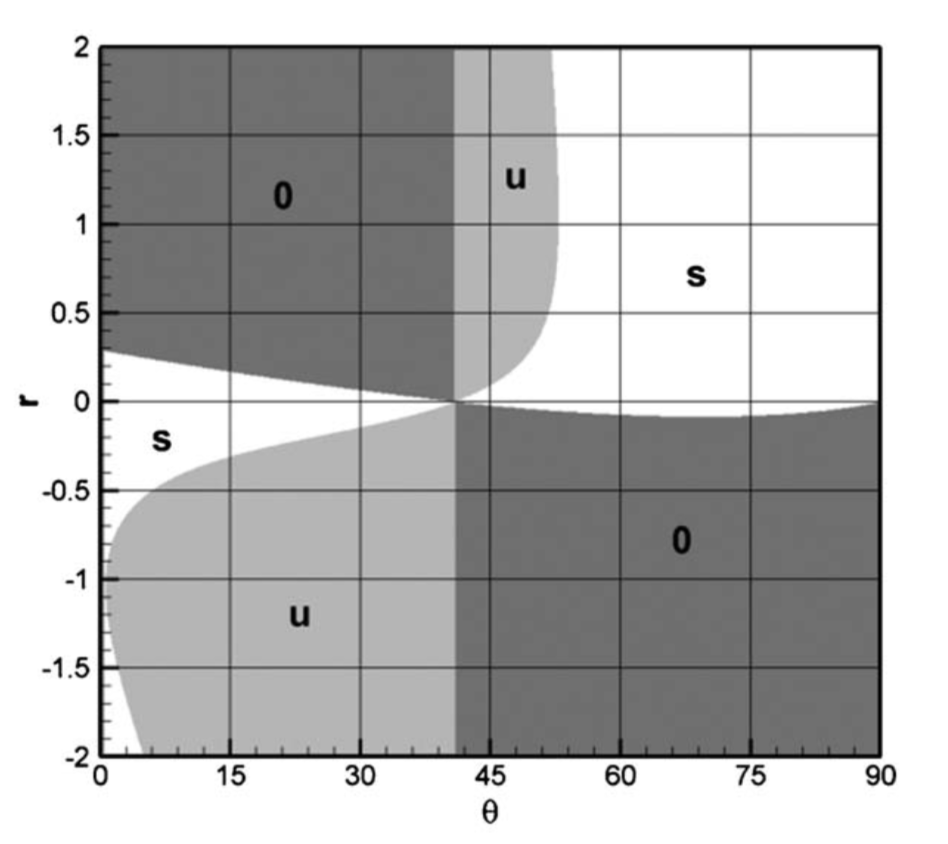
\includegraphics[width=210]{images_autres/cartebat.png}
\caption{Modèle du disque d'Euler étudié par Batista \cite{Batista}. La carte de stabilité indique si pour chaque couple $(\theta, r)$, le mouvement est stable (s), instable en cas de perturbation (u) ou si l'équilibre dynamique ne peut pas exister (0). $\theta$ décrit l'inclinaison de la roue et $r$ correspond au rayon des cercles décrits par le disque lorsqu'il roule sur sa tranche.}
\label{fig:figures}
\end{figure}

\section{Elasticité et saut d'une roue Cyr}
\subsection{Elasticité}
Afin d’étudier le stockage d’énergie élastique dans la roue lorsqu’elle est comprimée par une force verticale exercée selon son diamètre, nous avons besoin de calculer la flèche imposée par la force en question. Roark \cite{roark} développe des formules pour différents cas de chargement d’un anneau élastique, permettant entre autres de calculer les variations de diamètre horizontal et vertical en fonction des forces auxquelles l’anneau est soumis. \\
Il développe également toutes les formules nécessaires au calcul des contraintes dans la roue pour diverses géométries de section.

\subsection{Saut}
 Yang et Kim \cite{yangkim} étudient le comportement d'anneaux de diamètres millimétriques, faits de polyimides ou d'acier et de sections variables, comprimés puis relâchés. Leur saut est capturé par une caméra haute vitesse. Les résultats sont traités sous forme d'études adimensionnelles centrées sur l'énergie et la hauteur maximale de saut, $H_{max}$, puis confrontés à un modèle théorique développé à partir d'un bilan d'énergie. 
 
 \begin{figure}[h]
\centering
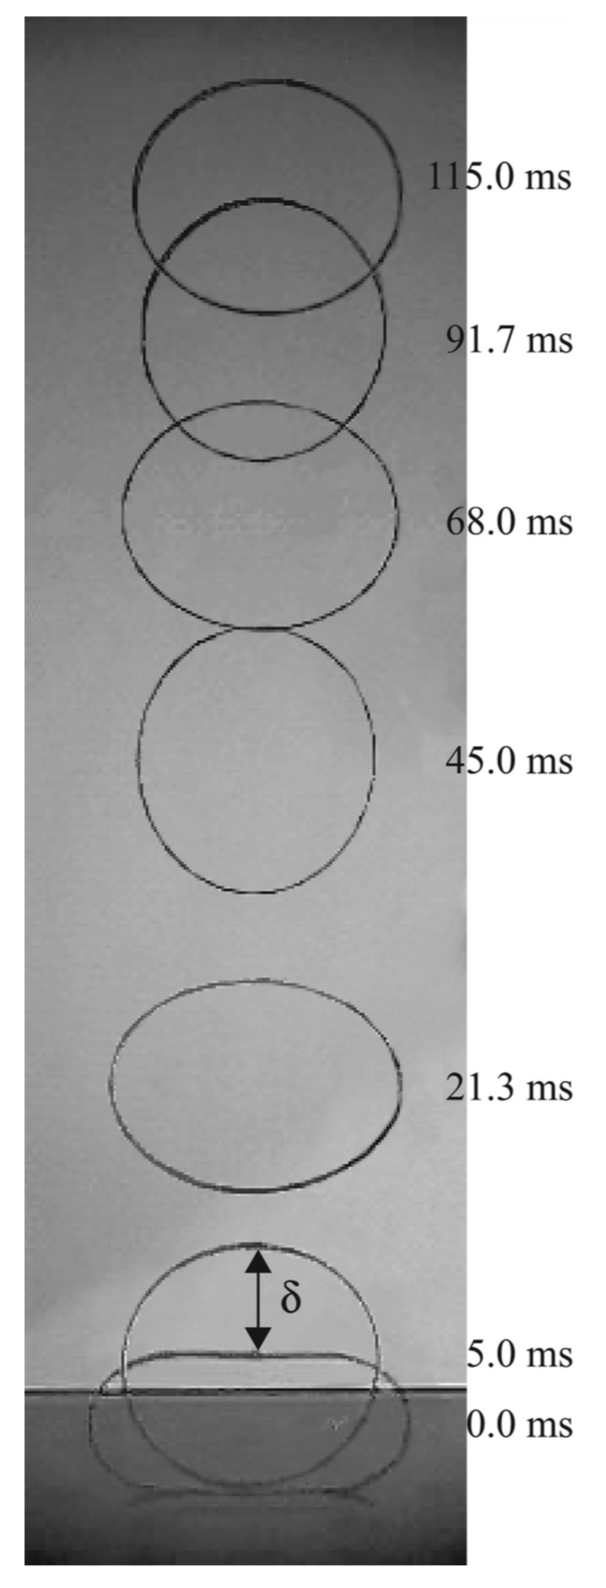
\includegraphics[width=80]{images_autres/yksaut.png}
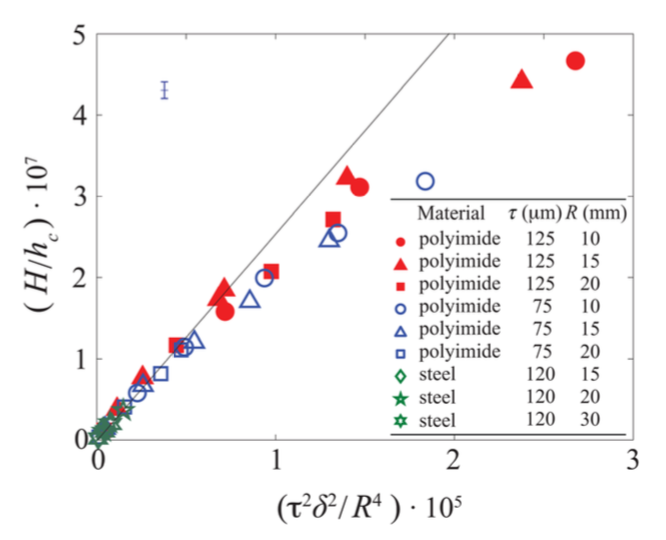
\includegraphics[width=260]{images_autres/ykres.png}
\caption{Saut d'un anneau élastique enregistré par vidéo lors d'une expérience avec un anneau en polyimide de rayon $R=16mm$, d'épaisseur $\tau=125\mu m$ et une déformation initiale de $\delta=14mm$. La figure de droite présente les résultats obtenus pour différents anneaux, sous forme de grandeurs adimensionnelles. $h_c=E/\rho g$ où $E$ est le module d'Young du matériau considéré et $\rho$ sa masse volumique \cite{yangkim}.}
\label{fig:figures}
\end{figure}